\documentclass[a4paper,twoside]{article}

\usepackage[T1]{fontenc}
\usepackage{epsfig}
\usepackage{subcaption}
\usepackage{calc}
\usepackage{amssymb}
\usepackage{amstext}
\usepackage{amsmath}
\usepackage{amsthm}
\usepackage{multicol}
\usepackage{pslatex}
\usepackage{apalike}
\usepackage[bottom,hang,flushmargin]{footmisc} % added hang,flushmargin
\usepackage{csquotes}

% OWN PACKAGES
\usepackage{microtype}
\usepackage{numprint}
\usepackage{tabularx}
\usepackage{balance}

\usepackage[table]{xcolor}
\usepackage{calc}
\usepackage{tikz}
\usetikzlibrary{calc,positioning,spy,shapes}


\tikzset{thick/.style = {line width = 1.0pt}}

\newlength{\pfull}  \setlength{\pfull}  {2mm}
\newlength{\phalf}  \setlength{\phalf}  {0.5\pfull}

\newlength{\lwffp}   \setlength{\lwffp}   {0.5000\dimexpr(\linewidth-1.0\pfull)}
\newlength{\lwfffp}  \setlength{\lwfffp}  {0.3333\dimexpr(\linewidth-2.0\pfull)}
\newlength{\lwffffp} \setlength{\lwffffp} {0.2500\dimexpr(\linewidth-3.0\pfull)}
\newlength{\lwfffffp}\setlength{\lwfffffp}{0.2000\dimexpr(\linewidth-4.0\pfull)}

\newlength{\twffp}   \setlength{\twffp}   {0.5000\dimexpr(\textwidth-1.0\pfull)}
\newlength{\twfffp}  \setlength{\twfffp}  {0.3333\dimexpr(\textwidth-2.0\pfull)}
\newlength{\twffffp} \setlength{\twffffp} {0.2500\dimexpr(\textwidth-3.0\pfull)}
\newlength{\twfffffp}\setlength{\twfffffp}{0.2000\dimexpr(\textwidth-4.0\pfull)}

\tikzstyle{labelStyle} = [ shape = rectangle, font = \scriptsize, text depth = 0, fill = white, inner sep = 4pt ]
\tikzstyle{labelN}  = [ labelStyle, anchor = north ]
\tikzstyle{labelNW} = [ labelStyle, anchor = north west ]
\tikzstyle{labelNE} = [ labelStyle, anchor = north east ]
\tikzstyle{labelS}  = [ labelStyle, anchor = south ]
\tikzstyle{labelSW} = [ labelStyle, anchor = south west ]
\tikzstyle{labelSE} = [ labelStyle, anchor = south east ]

\tikzstyle{figRC} = [shape = rectangle, rounded corners = 2mm, clip] % figure with Rounded Corners
\tikzstyle{spyRC} = [shape = rectangle, rounded corners = 2mm, %
    white, connect spies, every spy on node/.append style = {thick}] % spy with Rounded Corners
\tikzstyle{figNS} = [inner sep = 0pt, outer sep = 0pt] % figure with No Separators


\newcommand*\rot{\rotatebox{90}}
\newcommand{\rott}[2]{\multicolumn{1}{#1}{\rot{#2}}}


\usepackage[hidelinks]{hyperref}

% Define starred commands
\usepackage{xparse}

% Enumerations
\usepackage[inline]{enumitem}

% Draw figures
% \usepackage{tikz}
% \includegraphs for .tikz files
\usepackage{tikzscale}

% Lay out multiple figures
\usepackage{subcaption}

% Extended control of figure positioning
\usepackage{dblfloatfix}

\usepackage{float}
\newfloat{lstfloat}{htbp}{lop}
\floatname{lstfloat}{Listing}
\def\lstfloatautorefname{Listing} % needed for hyperref/auroref

% Algorithms
\usepackage[noend,noline,boxed]{algorithm2e}
\SetAlCapSkip{1em}
% Python style
\DontPrintSemicolon
\SetStartEndCondition{ }{}{}%
\SetKwIF{If}{ElseIf}{Else}{if}{:}{else if}{else}{end if}%
\SetKwFor{For}{for}{:}{next}%
\SetKw{kwYield}{yield}

% Source code listings
\usepackage{listings}
\usepackage{lstset-typescript}

% Underlined text with linebreaks
\usepackage[normalem]{ulem}

% SI units
\usepackage{siunitx}
\sisetup{input-ignore={,},input-decimal-markers={.}}  % allow for manual thousands separators in numbers
\sisetup{group-separator = {,}}
\DeclareSIUnit\bit{bit}
\DeclareSIUnit\byte{B}

\usepackage{xcolor}

% Convenient references (needs to be loaded after algorithms)
\usepackage[nameinlink]{cleveref}

% Tables
\usepackage{booktabs}
\usepackage{multirow}

\usepackage{makecell}
\renewcommand\theadalign{bc}

\usepackage{threeparttable}

% Bar charts
\usepackage{bchart}

\definecolor{plots-1}{RGB}{228,26,28}
\definecolor{plots-2}{RGB}{55,126,184}

\usepackage{tikz}
\usetikzlibrary{calc,fit,backgrounds,positioning,shapes,snakes,arrows.meta,spy,shapes.multipart,patterns}

\usepackage{pgfplots}
\usepackage{pgfplotstable}
\usepackage{pgfplotstablefilter}
\pgfplotsset{compat=newest}% es muss mindestens Version 1.8 installiert sein
\usepgfplotslibrary{statistics}



% END OWN PACKAGES

\usepackage{SCITEPRESS}     % Please add other packages that you may need BEFORE the SCITEPRESS.sty package.


% Semantic markup
\newcommand\caps[1]{%
	\textsc{#1}%
}
\NewDocumentCommand\mycode{sm}{%
    \IfBooleanTF#1%
        {{\small\texttt{#2}}}% If a star is seen
        {{\small\texttt{\detokenize{#2}}}}%     If no star is seen
}

% Semantic mathmode markup
\newcommand{\mli}[1]{\mathit{#1}}
\newcommand{\mtx}[1]{\text{#1}}

% Todo comments
\newcommand\TODO[1]{%
    {\leavevmode\bfseries\color{red}#1}%
}

% bchart legends
% CREDITS: https://tex.stackexchange.com/a/379816/221054
\usetikzlibrary{fit}

\makeatletter
\newdimen\legendxshift
\newdimen\legendyshift
\newcount\legendlines
% distance of frame to legend lines
\newcommand{\bclldist}{1mm}
\newcommand{\bclegend}[3][10mm]{%
    % initialize
    \legendxshift=0pt\relax
    \legendyshift=0pt\relax
    \xdef\legendnodes{}%
    % get width of longest text and number of lines
    \foreach \lcolor/\ltext [count=\ll from 1] in {#3}%
        {\global\legendlines\ll\pgftext{\setbox0\hbox{\bcfontstyle\ltext}\ifdim\wd0>\legendxshift\global\legendxshift\wd0\fi}}%
    % calculate xshift for legend; \bcwidth: from bchart package; \bclldist: from node frame, inner sep=\bclldist (see below)
    % \@tempdima: half width of bar; 0.72em: inner sep from text nodes with some manual adjustment
    \@tempdima#1\@tempdima0.5\@tempdima
    \pgftext{\bcfontstyle\global\legendxshift\dimexpr\bcwidth-\legendxshift-\bclldist-\@tempdima-0.72em}
    % calculate yshift; 5mm: heigt of bar
    \legendyshift\dimexpr5mm+#2\relax
    \legendyshift\legendlines\legendyshift
    % \bcpos-2.5mm: from bchart package; \bclldist: from node frame, inner sep=\bclldist (see below)
    \global\legendyshift\dimexpr\bcpos-2.5mm+\bclldist+\legendyshift
    % draw the legend
    \begin{scope}[shift={(\legendxshift,\legendyshift)}]
    \coordinate (lp) at (0,0);
    \foreach \lcolor/\ltext [count=\ll from 1] in {#3}%
    {
        \node[anchor=north, minimum width=#1, minimum height=5mm,fill=\lcolor] (lb\ll) at (lp) {};
        \node[anchor=west] (l\ll) at (lb\ll.east) {\bcfontstyle\ltext};
        \coordinate (lp) at ($(lp)-(0,5mm+#2)$);
        \xdef\legendnodes{\legendnodes (lb\ll)(l\ll)}
    }
    % draw the frame
    \node[draw, inner sep=\bclldist,fit=\legendnodes] (frame) {};
    \end{scope}
}
\makeatother

% Properly spaces tnotes for threeparttable
% CREDITS: https://tex.stackexchange.com/a/108640/221054
% This is like `\tnote`, but uses the space of the argument
\newcommand\stnote[1]{\textsuperscript{\TPTtagStyle{#1}}}

% Alpha numbers for threeparttable tnotes
\makeatletter
\newcommand{\alphtnotetext}[1]{\itshape \@alph{#1}}
\makeatother
\newcommand{\alphtnote}[1]{\stnote{\alphtnotetext{#1}}}

\definecolor[named]{ACMBlue}{cmyk}{1,0.1,0,0.1}
\definecolor[named]{ACMYellow}{cmyk}{0,0.16,1,0}
\definecolor[named]{ACMOrange}{cmyk}{0,0.42,1,0.01}
\definecolor[named]{ACMRed}{cmyk}{0,0.90,0.86,0}
\definecolor[named]{ACMLightBlue}{cmyk}{0.49,0.01,0,0}
\definecolor[named]{ACMGreen}{cmyk}{0.20,0,1,0.19}
\definecolor[named]{ACMPurple}{cmyk}{0.55,1,0,0.15}
\definecolor[named]{ACMDarkBlue}{cmyk}{1,0.58,0,0.21}

\colorlet{paperbackground}{white}
\colorlet{accent1}{ACMBlue}
\colorlet{accent2}{ACMYellow}
\colorlet{accent3}{ACMOrange}
\colorlet{accent4}{ACMRed}
\colorlet{accent5}{ACMLightBlue}
\colorlet{accent6}{ACMGreen}
\colorlet{accent7}{ACMPurple}
\colorlet{accent8}{ACMDarkBlue}

\colorlet{bchart.accent1}{accent1!70!paperbackground}
\colorlet{bchart.accent2}{accent2!70!paperbackground}
\colorlet{bchart.accent3}{accent3!70!paperbackground}
\colorlet{bchart.accent4}{accent4!70!paperbackground}
\colorlet{bchart.accent5}{accent5!70!paperbackground}
\colorlet{bchart.accent6}{accent6!70!paperbackground}
\colorlet{bchart.accent7}{accent7!70!paperbackground}
\colorlet{bchart.accent7}{accent7!70!paperbackground}
\colorlet{bchart.accent8}{accent8!70!paperbackground}


\lstset{frame=none,
	showstringspaces=false,
	columns=flexible,
	basicstyle={\small\ttfamily},
	numbers=none,
	keywordstyle=\textbf,
	stringstyle=\color{blue},
	breaklines=true,
	breakatwhitespace=true,
	tabsize=3
}


\colorlet{punct}{black}
\definecolor{delim}{RGB}{20,105,176}
\colorlet{numb}{magenta!60!black}
\lstdefinelanguage{json}{
    frame=lines,
    literate=
     *{0}{{{\color{numb}0}}}{1}
      {1}{{{\color{numb}1}}}{1}
      {2}{{{\color{numb}2}}}{1}
      {3}{{{\color{numb}3}}}{1}
      {4}{{{\color{numb}4}}}{1}
      {5}{{{\color{numb}5}}}{1}
      {6}{{{\color{numb}6}}}{1}
      {7}{{{\color{numb}7}}}{1}
      {8}{{{\color{numb}8}}}{1}
      {9}{{{\color{numb}9}}}{1}
      {:}{{{\color{punct}{:}}}}{1}
      {,}{{{\color{punct}{,}}}}{1}
      {\{}{{{\color{delim}{\{}}}}{1}
      {\}}{{{\color{delim}{\}}}}}{1}
      {[}{{{\color{delim}{[}}}}{1}
      {]}{{{\color{delim}{]}}}}{1},
}

\lstdefinelanguage{sourcegraph}{
	alsodigit={-},
	morekeywords={
		count,
		file,
		-file,
		select
	},
	literate=*{\\.}{{{\color{accent4}{\textbackslash.}}}}{1},
	moredelim=[is][\textbf]{\ }{:},
	% placeholders
	moredelim=[s][\color{accent1}\itshape]{<}{>},  % TODO: italic does not work
	morestring=[b]
}


% Left-align footnotes in minipages - this reverts a part of the acm style
% CREDITS: https://github.com/borisveytsman/acmart/issues/449#issuecomment-932653376
\makeatletter
\long\def\@mpfootnotetext#1{%
\global\setbox\@mpfootins\vbox{%
  \unvbox\@mpfootins
  \reset@font\footnotesize
  \hsize\columnwidth
  \@parboxrestore
  \protected@edef\@currentlabel
	   {\csname p@mpfootnote\endcsname\@thefnmark}%
  \color@begingroup%\centering - commented out centering footnotes
	\@makefntext{%
	  \rule\z@\footnotesep\ignorespaces#1\@finalstrut\strutbox}%
  \color@endgroup}}
\makeatother

\newcommand\footnoteseparator{\textsuperscript{,}}

\crefname{requirement}{requirement}{requirements}
\crefname{question}{question}{questions}


\begin{document}

\title{Augmenting Library Development by Mining Usage Data from~Downstream~Dependencies}

\author{\authorname{Christoph Thiede, Willy Scheibel, Daniel Limberger, and J{\"u}rgen D{\"o}llner}
\affiliation{Hasso Plattner Institute, Digital Engineering Faculty, University of Potsdam}}

\keywords{Mining Software Repositories, Downstream Dependencies, API Usage.}

\inofficialcopyrightnotice{Author's Version. This paper has been published in the Proceedings of the 17th International Conference on Evaluation of Novel Approaches to Software Engineering -- ENASE, 221--232, 2022, and is accessible on \textsc{SciTePress}: \url{https://doi.org/10.5220/0011093700003176}}


\abstract{%
    Software and its dependencies build up a graph where edges connect packages according to their dependencies.
    In this graph, downstream dependencies are all the nodes that depend on a package of interest.
    Although gathering and mining such downstream dependencies allow for informed decision-making for a package developer, there is much room for improvement, such as automation and integration of this approach into their development process.
    This paper makes two contributions:
    \begin{enumerate*}[label=(\roman*)]
        \item We propose an approach for efficiently gathering downstream dependencies of a single package and extracting usage samples from them using a static type analyzer.
		\item We present a tool that allows npm package developers to survey the aggregated usage data directly in their IDE in an interactive and context-sensitive way.
	\end{enumerate*}
	We evaluate the approach and the tool on a selection of open source projects and specific development-related questions with respect to found downstream dependencies, gathering speed, and required storage.
    Our methods return over \numprint{8000} downstream dependencies for popular packages and process about 12 dependencies per minute.
    The usage sample extraction offers high precision for basic use cases.
    The main limitations are the exclusion of unpopular and closed-source downstream dependencies as well as failing analysis when encountering complex build configurations or metaprogramming patterns.
    To summarize, we show that the tool supports package developers in gathering usage data and surveying the use of their packages and APIs within their downstream dependencies, allowing for informed decision-making and improving the resdesign of APIs.
}



\onecolumn \maketitle \normalsize \setcounter{footnote}{0} \vfill


\section{Introduction}
\label{sec:introduction}

The continued proliferation and improvement of open-source software (OSS) platforms such as \emph{GitHub} or \emph{GitLab} and package deployment ecosystems such as \emph{npm}, \emph{pip}, or \emph{NuGet} support and facilitate software development on a global scale.
Open-source development offers many advantages over traditional closed-source development, including voluntary contributions from the open-source community, greater transparency in security-related areas, and a high potential for solution reuse~\cite{saied2018-reusability}.
These solutions are typically organized as packages, each solving an isolated problem and providing a higher-level interface.
Packages can \emph{depend} on existing packages by including them in their manifest, i.e., the \texttt{package.json} file of npm packages or the \texttt{requirements.txt} file of Python projects.
These dependency relations form a large directed graph connecting significant parts of the software world for today's programming language ecosystems.
We define a software ecosystem as a collection of software projects, which are developed and which co-evolve in the same environment.

Despite this connectedness by design, however, the development process of many packages is still characterized by an isolated approach:
While OSS developers commonly submit tickets to or contribute patches against \emph{upstream repositories} that they depend on to solve subproblems, the reverse direction of these edges -- called \emph{downstream dependencies} and in the following referred to as \emph{dependencies} -- is often neglected by package developers.
This deficit can cause a wide range of alignment issues, including poorly suited interfaces~\cite{piccioni2013empirical}, unidentified defects~\cite{wong2017more}, and compatibility problems~\cite{bogart2015breaks}.
Eventually, all these issues impair the capabilities of the global OSS community to build and support high-quality packages.

To tackle these concerns, we propose an approach to extract API usage samples from downstream-dependency repositories of individual packages to support package developers in exploring usages of their packages.
We make these data directly available to package developers by integrating them into an integrated development environment (IDE).

Our approach consists of three steps:
\begin{enumerate*}[label=(\roman*)]
	\item collect downstream dependency repositories from public source code repositories,
	\item mine package usage samples from these dependencies using a type analyzer,
	and \item aggregate and present these usage data to the package developer in its development environment.
\end{enumerate*}
The approach is implemented as a Visual Studio Code extension\footnote{All presented artifacts are available on GitHub: \href{https://github.com/LinqLover/downstream-repository-mining}{https://github.com/LinqLover/downstream-repository-mining}~\cite{thiede2022dowdep}} and evaluated on a selection of open source projects and specific development-centric questions.

The remainder of this paper is structured as follows:
In \cref{sec:related_work}, we summarize existing approaches and in \cref{sec:approach}, we outline the overall conditions for our solution and detail the collection of downstream dependency repositories and subsequent mining of usage data.
In \cref{sec:implementation}, we present an implementation of our approach and outline design decisions for displaying usage samples to the user.
Finally, in \cref{sec:evaluation}, we examine the fitness of our data mining approach and the usability of the display solution.
\Cref{sec:conclusion} concludes this paper.




\section{Related Work}
\label{sec:related_work}
%
Proper tooling design for improving package developers' knowledge about interface usages in dependencies has not yet attracted significant attention in the scientific community.
Nevertheless, programmatic analysis of dependency graphs and API usage mining are already standard techniques in the field of \emph{mining software repositories} (MSR).
Chaturvedi et al. provide a broad overview of existing achievements and ongoing research topics in this field~\cite{chaturvedi2013tools}.
Besides source code repositories, they describe data sources worthwhile to examine, including telemetry data from IDEs, issue trackers, and discussion platforms, and propose different directions for evaluating the retrieved data, e.g., classifying or ranking repositories, analyzing the evolution of projects, studying development communities, but also inspecting the relationships and dependencies between projects.
We further consider related work in the areas of dependency graphs, usage sample extraction, and tooling support.


\paragraph{Searching dependency graphs.}
\label{sec:related_work/dependencies}
%
A common purpose for \emph{analyzing dependency graphs} is to discover transitive upstream dependencies of a project and assess their impact on the stability and vulnerability of the project~\cite{kikas2017structure}.
Similarly, the spreading of security vulnerabilities along the chain of downstream dependencies can be measured~\cite{decan2018impact}.

However, existing research on dependency graphs takes a broad statistical perspective and relies on a large corpus of downloaded software repositories~\cite{abdalkareem2017developers,kikas2017structure,katz2020libraries}.
As opposed to this approach, these capacities are not suitable for scenarios that developers of a single package occasionally perform.
In this case, developers will often use a public \emph{code search} service instead, such as \emph{GitHub} or \emph{Sourcegraph}.
Liu et al. provide a survey of methods and trends in code search tools that include newer approaches such as structural or semantic search queries, code similarity metrics, or machine learning methods~\cite{liu2020opportunities}.


\paragraph{Extracting usage samples.}
\label{sec:related_work/usage_samples}
%
Dependency graphs do not provide information about package usage at sufficient granularity. For example, insights about referencing package classes or methods are missing.
The process of extracting fine-grained information about all references to individual elements of an interface is referred to as \emph{API usage analysis}~\cite{lammel2011large}.
A simple approach is to perform a string search for package names or members in the dependencies~\cite{mileva2010mining}, or to operate on the \emph{abstract syntax tree} (AST) of each parsed dependency to avoid false positive caused by ambivalent identifier names~\cite{qiu2016understanding}.
In addition, one can collect usage data to analyze the historical importance of certain features supported by an API~\cite{sawant2017fine}.

However, the precision of ASTs is limited for \emph{dynamically typed} languages such as JavaScript or Python.
As opposed to static typing, the value type of an expression in a dynamically typed language may be unknown at the compile time of the program.
For this reason, a \emph{type analysis} can help to predict runtime types of all expressions in the AST~\cite{jensen2009type}.
This is usually accomplished by analyzing the control flow of a program and inferring possible types of every variable or function.
Another source for enhancing type information is \emph{call graphs} that are either gathered \emph{statically}, i.e., as a result of a theoretical analysis of the source code, or \emph{dynamically}, i.e., sampled during actual program execution.
While the latter method is better suited to include more contextual information, the former method has the advantage that it can be applied to a more considerable amount of source code without requiring concrete entry points, parameterization, and run-time data.
Many solutions exist that analyze the structure of programs and extract relevant information to build call graphs:

Collard et al. propose an infrastructure called \caps{srcML} that aims to create a unified representation of multilingual source code snippets for arbitrary analysis purposes, including the construction of call graphs~\cite{collard2013srcml}.
Another solution utilizes an island parser to build polyglot call graphs~\cite{bogar2018lightweight}.
Furthermore, Antal et al. compare several call graph generators for JavaScript and emphasize that static call graph generators have limited precision by design for languages supporting dynamic typing or meta-programming mechanisms~\cite{antal2018static}.

To merge dependency graphs and call graphs, ecosystem call graphs can be constructed by applying call graphs to entire ecosystems that cross repository boundaries.
Many approaches apply this concept to different ecosystems, often aiming to conduct fine-grained impact analysis for security vulnerabilities~\cite{hejderup2018software,boldi2020fine,wang2020empirical,hejderup2021praezi,keshani2021scalable,nielsen2021modular}.
Another approach is the \emph{precise code intelligence} feature of Sourcegraph, which makes code references explorable across repository boundaries for repositories that provide a metadata file in the \emph{Language Server Index Format}.\footnote{\url{https://docs.sourcegraph.com/code_intelligence/explanations/precise_code_intelligence}}

After collecting these usage data, additional processing is possible to extract general usage information from the extensive raw data.
Next to basic grouping and counting operations, such aggregations can be built by detecting popular \emph{usage patterns} of API features in the downstream dependencies.
Zhong et al. propose such a framework, that, for instance, finds sequences of API members that are invoked frequently and even uses these patterns for guiding API users by giving them recommendations~\cite{zhong2009mapo}.
Hanam et al. pursue a different goal in their tool that helps package developers assess the impact of breaking API changes on the functionality of downstream dependencies~\cite{hanam2019aiding}.

\paragraph{Presentation of results.}
\label{sec:related_work/presentation}

To establish an adequate developer experience, any collected usage data still need to be presented suitably.
Due to the hierarchical structure of source code, a common approach for this is a hierarchical and navigatable representation of the collected call tree.
An early form of this representation has been invented as the interactive \enquote{message set} tool for browsing senders and implementors in an object-oriented system for the Smalltalk programming environment \cite{goldberg1984smalltalk}.
Modern alternatives include the \emph{Stacksplorer} \cite{karrer2011stacksplorer} or \emph{Blaze} \cite{kramer2012blaze} that list next to the currently focused method other methods which are adjacent to this method in the call graph.
With a focus on exploring references to API members, De Roover et al. propose a set of additional views, including hierarchical lists and word clouds for highly referenced identifiers \cite{de2013multi}.
Focusing on exploring APIs in a non-code-centric way, Hora and Valente propose a dashboard that allows developers to browse existing APIs and track possibly breaking changes in their interfaces \cite{hora2015apiwave}.



\section{Downstream Dependency Mining}
\label{sec:approach}
%
Our approach to improve developers' knowledge about the usage of their packages is based on the automatic gathering of downstream dependency information and integration into their development environment. This approach assumes a target package and focuses on showing a developer actual usage of parts of their package and, in particular, answering the following questions:
In doing so, we identified three questions from package developers about the usage of their packages:
%
\begin{enumerate}[label=Q\arabic*]
	\item \label[question]{q1} Which dependencies are using the target package, and what problems do they try to solve with them?
	\item \label[question]{q2} By how many dependencies is a particular package member being used?
	\item \label[question]{q3} In which contexts and constellations is a particular package member being used?
\end{enumerate}
%
For an effective integration into the development process, we pose three non-functional requirements:
%
\begin{enumerate}[label=R\arabic*]
	\item \label[requirement]{req1} The tool is ready to use out of the box and requires little configuration (less than 5 minutes for a new user).
	\item \label[requirement]{req2} The tool consumes sufficiently few computational resources to run on a single machine but still delivers interactive response times according to Shneiderman's requirement to frequent tasks~\cite{shneiderman2010designing}.
	\item \label[requirement]{req3} The tool blends in with the usual workflow of package developers at the best possible rate.
\end{enumerate}
%
On a conceptual level, we separate the approach into the collection of downstream dependency projects and mining of usage samples based on a target package.

\begin{algorithm*}[t]
	\caption{Extraction of usage samples.}\label{alg:usage_mining}

	\KwIn{\\\Indp
		$\mli{package}$: target package \\
		$\mli{dependencies}$: downstream dependencies}
	\KwOut{usage samples (set of strings)}
	\;
	\For{$\mli{dependency} \in \mli{dependencies}$}{
		$\mli{asf} \gets \mtx{parse}(\mli{dependency} \cup \mli{package})$\;
	  	$\mtx{annotate\_types}(\mli{asf})$\;
		\For{$\mli{ast} \in \mli{asf}$}{
			\For{$\mli{node} \in \mli{dfs}(\mli{ast})$}{
				\For{$\mli{pattern} \in \mli{patterns}$}{
					\If{$\mli{pattern}.\mtx{matches}(\mli{node}) \wedge\, \mli{package}.\mtx{declares}(\mli{pattern}.\mtx{getType}(\mli{node}))$}{
						\kwYield{$\mli{node}.\mtx{text}$}
					}
				}
			}
		}
	}
\end{algorithm*}

\subsection{Downstream Dependency Collection}
\label{sec:approach/dependency_collection}

In the first step, a list of repositories that depend on the target package has to be assembled.
As mentioned in \cref{sec:related_work/usage_samples}, many approaches start with a large downloaded corpus of unspecific repositories from the ecosystem, which they then iterate over to filter the relevant repositories.
However, a major drawback of this approach is the high resource demand for both creating and traversing this corpus.
This approach is suited for analyzing repositories on a large scale but is not conform to \cref{req1} because of its large footprint in terms of computational power, memory, and time.
As an alternative, we have decided to apply filtering to the set of repositories before downloading a subset of it to the developers' machine.
For that, we use two types of data sources that are available as public web platforms:

\begin{enumerate}[label=(\roman*)]
	\item Package repositories that maintain a doubly-connected edge list of interdependent packages in an ecosystem.
	\item Code search engines that index the source code of many repositories from OSS platforms. Using these search engines, we can query all repositories that declare a dependency on the target package in their package manifest file.
\end{enumerate}

\subsection{Usage Sample Mining}
\label{sec:approach/usage_mining}

Having downloaded the selected downstream dependency repositories, the next step is to extract usage samples for the target package from each dependency repository.
Our goal is to gather fine-grained source code excerpts that reference individual identifiers exposed by the target package.
The complete procedure is displayed in \cref{alg:usage_mining}.

%
To do so, the source code of every dependency repository as well as the source code of the target package are parsed, each into a separate \emph{abstract syntax forest} (ASF, i.e., a set of ASTs).
In a second step, static type analysis against each dependency ASF is performed together with the target package's ASF.
The results of the type analysis are attached to the ASF so that every identifier is annotated with a type symbol that links to the declaration of the type for the identifier.
For instance, after this step, every variable node contains a link to the assignment node of this variable, and every function call expression contains a link to the definition of this function.
The operating principle of this type analysis depends on the kind of programming language.
In statically typed languages, type symbols can be retrieved from declarations, whereas in dynamically typed languages, a control flow analysis will be required to identify the origin of every identifier's type.

In the final step, all nodes whose type is declared in the target package are collected from each ASF.
To identify these links, we use a set of language-specific patterns for AST subtrees that constitute a usage expression.
In particular, each of these patterns expects a node containing a link to an identifier declaration (see \cref{fig:approach/usage_mining/patterns}).



\begin{figure*}
	\begin{minipage}{\linewidth}
		\colorlet{lowlight}{black!40}
		\newcommand\textlowlight[1]{\textcolor{lowlight}{#1}}
		\newcommand\texthighlight[1]{\textbf{\textcolor{accent1}{#1}}}
		\begin{center}
			\begin{subfigure}[t]{.30\linewidth}
				\begin{tikzpicture}
                	\node {CallExpression}
                		child {node [accent1] {\textbf{identifier}}}
                		child [lowlight] {node [lowlight, yshift = -0.5cm] {typeArguments}}
                		child [lowlight] {node [lowlight] {arguments}};
                \end{tikzpicture}
                \caption[LoF entry]{
                	Node pattern for a TypeScript function call, such as in:

                	\mycode*{\textlowlight{result = }\uline{\texthighlight{fun}<\textlowlight{T1}, \textlowlight{T2}>(\textlowlight{arg1}, \textlowlight{arg2})}\textlowlight{;}}
                }

			\end{subfigure}
			\hfill
			\begin{subfigure}[t]{.30\linewidth}
				\begin{tikzpicture}
                	\node {PropertyAccessExpression}
                		child {node [accent1] {\textbf{identifier}}}
                		child [white] {node [yshift = -0.5cm] {\phantom{node}}}  % ensure same height as sibling figures
                		child [lowlight] {node [lowlight] {name}}
                		;
                \end{tikzpicture}
                \caption[LoF entry]{
                	Node pattern for a JavaScript property access, such as in:

                	\mycode*{\textlowlight{return }\uline{\textlowlight{obj}.\texthighlight{prop}}\textlowlight{;}}
                }

			\end{subfigure}
			\hfill
			\begin{subfigure}[t]{.30\linewidth}
				\begin{tikzpicture}
                	\node [accent1] {\textbf{JsxOpeningExpression}}
                		child [lowlight] {node [lowlight] {tagName}}
                		child [lowlight] {node [lowlight, yshift = -0.5cm] {typeArguments}}
                		child [lowlight] {node [lowlight] {attributes}};
                \end{tikzpicture}
                \caption[LoF entry]{
                	Node pattern for a JSX opening element (as supported in React or TypeScript), such as in:

                	\mycode*{\textlowlight{elem = }\uline{<\texthighlight{Button} \textlowlight{color}="\textlowlight{blue}"> \textlowlight{Submit</Button>}}\textlowlight{;}}
                }
			\end{subfigure}

            \vspace{\baselineskip}
			\caption{AST patterns for example JavaScript/TypeScript expressions.
				The \texthighlight{highlighted} node contains the link to the declaration of the referenced identifier.
			}
			\label{fig:approach/usage_mining/patterns}
		\end{center}
	\end{minipage}
\end{figure*}

\section{Prototype}
\label{sec:implementation}

In our prototype, we focus on analyzing JavaScript projects for node.js.
This decision is motivated by the large prevalence of JavaScript\footnote{GitHut 2.0: A small place to discover languages in GitHub. \url{https://madnight.github.io/githut/\#/pushes}} as well as the first-rate extent of the npm ecosystem which has been unsurpassed since 2015\footnote{Modulecounts: \url{http://www.modulecounts.com/}}.
The prototype instantiates the downstream dependency collection and the usage sample mining and allows for the integration of the results into the development environment.

\subsection{Downstream Dependency Collection}
\label{sec:implementation/dependency_collection}

The de-facto standard package repository manager for node.js is npm.
To fetch downstream dependency packages from the npm registry, we use the npm package \texttt{npm-dependants} which scrapes the dependents list from npmjs.com as there does not exist a publicly available API for these data.
To keep the footprint of our implementation small, only a part of the dependents list is scraped.
Then, basic metadata for each found package is requested from the npm registry, including the \emph{tarball} URL of the latest package version, using the package \mycode{package-metadata}.
Finally, each tarball is downloaded and extracted using the package \mycode{download-package-tarball}.

\begin{lstfloat}[t]
\begin{lstlisting}[language=typescript,%json,
	label=sec:implementation/package.json,
	caption={Example \texttt{package.json} file for the \texttt{ripple-lib} package specifying multiple dependencies (truncated). The list of dependencies that are extracted from this example contains \texttt{bignumber.js}, \texttt{https-proxy-agent}, and \texttt{jsonschema}.}]
{
	"name": "ripple-lib",
	"version": "1.10.0",
	"description": "An API for the XRP Ledger",
	"dependencies": {
		"bignumber.js": "^9.0.0",
		"https-proxy-agent": "^5.0.0",
		"jsonschema": "1.2.2"
	}
}
\end{lstlisting}
\end{lstfloat}

For the second method -- based on a code search engine --, we have identified Sourcegraph\footnote{\url{https://sourcegraph.com/}} as a promising platform.
npm packages specify their dependencies in a \mycode{package.json} metadata file (see \cref{sec:implementation/package.json}).
To find all packages depending on a certain package, we can search all available \mycode{package.json} files for a reference to this package identifier.
We refine our search query with some additional constraints to filter out package copies from \mycode{node_modules} folders that downstream developers have pushed accidentally, and to limit the number of results retrieved.
We submit this search query to the publicly available GraphQL API of Sourcegraph\footnote{\url{https://docs.sourcegraph.com/api/graphql}} by using the npm package \mycode{graphql-request}.
After retrieving a search result, we download a snapshot of the full repository by using the package \mycode{download-git-repo}.

Additionally, we enrich the metadata of each package with a few metrics indicating its popularity from the associated GitHub repository if specified.
The GitHub API is accessed via the official \emph{octokit} library\footnote{\url{https://octokit.github.io/}}.

\subsection{Usage Sample Mining}
\label{sec:implementation/usage_mining}

For parsing the dependencies, we use the \emph{TypeScript Compiler API}\footnote{\url{https://github.com/Microsoft/TypeScript/wiki/Using-the-Compiler-API}}.
TypeScript is an extension of JavaScript that adds strong typing; typing is based on a combination of implicit type inference and explicit type declarations.
As a side benefit, our implementation is also able to analyze packages implemented in true TypeScript.

The TypeScript compiler's \emph{binder} component annotates every node of the parsed program with a type symbol if it can resolve one.
After performing a type analysis of the dependency by instrumenting the binder, we collect all nodes from the type-annotated ASF that refer to the target package,
matching each node against a list of defined patterns (similar to \cref{fig:approach/usage_mining/patterns}).
A lookup of the node's type symbol's declaration is performed based on the syntax kinds of the node, its ancestors, and its descendants, and then compared with the source directory of the target package.

\begin{figure*}[t] % requires figures-spec.tex
    %
    \begin{tikzpicture}[figNS, spy using outlines = {style = spyRC, gray, magnification = 2.0, width = 48mm, height = 16mm}]
        % graphics:
        \node[figRC, anchor = east](fig0) at (0,0)
            {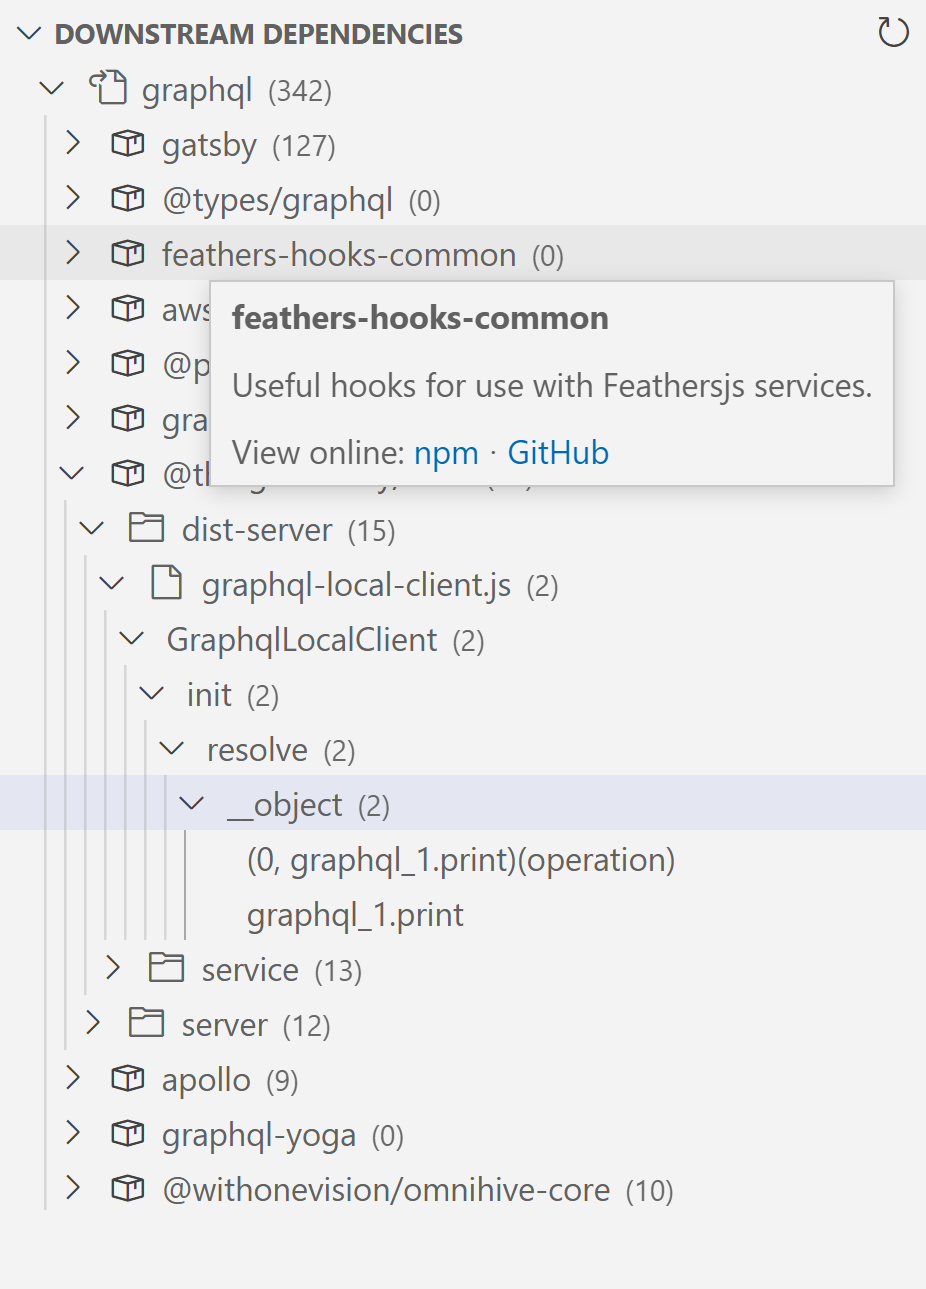
\includegraphics[width = 0.2857\dimexpr(\textwidth-2.0\pfull) - 0.25\pfull]{figures/dependencies-cropped}};
        \node[figRC, anchor = west](fig1) at ([xshift = \pfull] fig0.east)
            {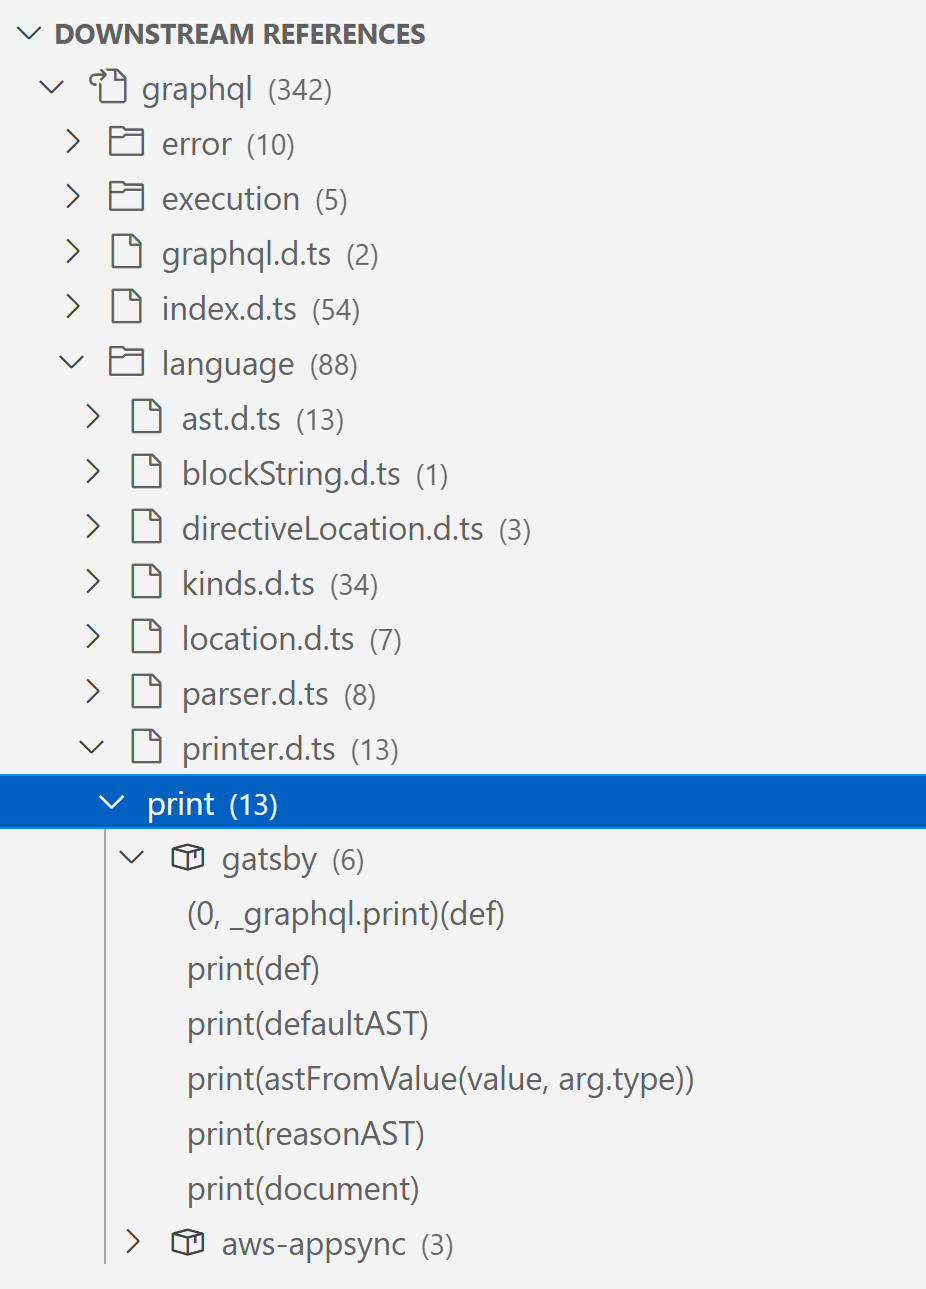
\includegraphics[width = 0.2857\dimexpr(\textwidth-2.0\pfull) - 0.25\pfull]{figures/references-cropped}};
        \node[figRC, anchor = west](fig2) at ([xshift = \pfull] fig1.east)
            {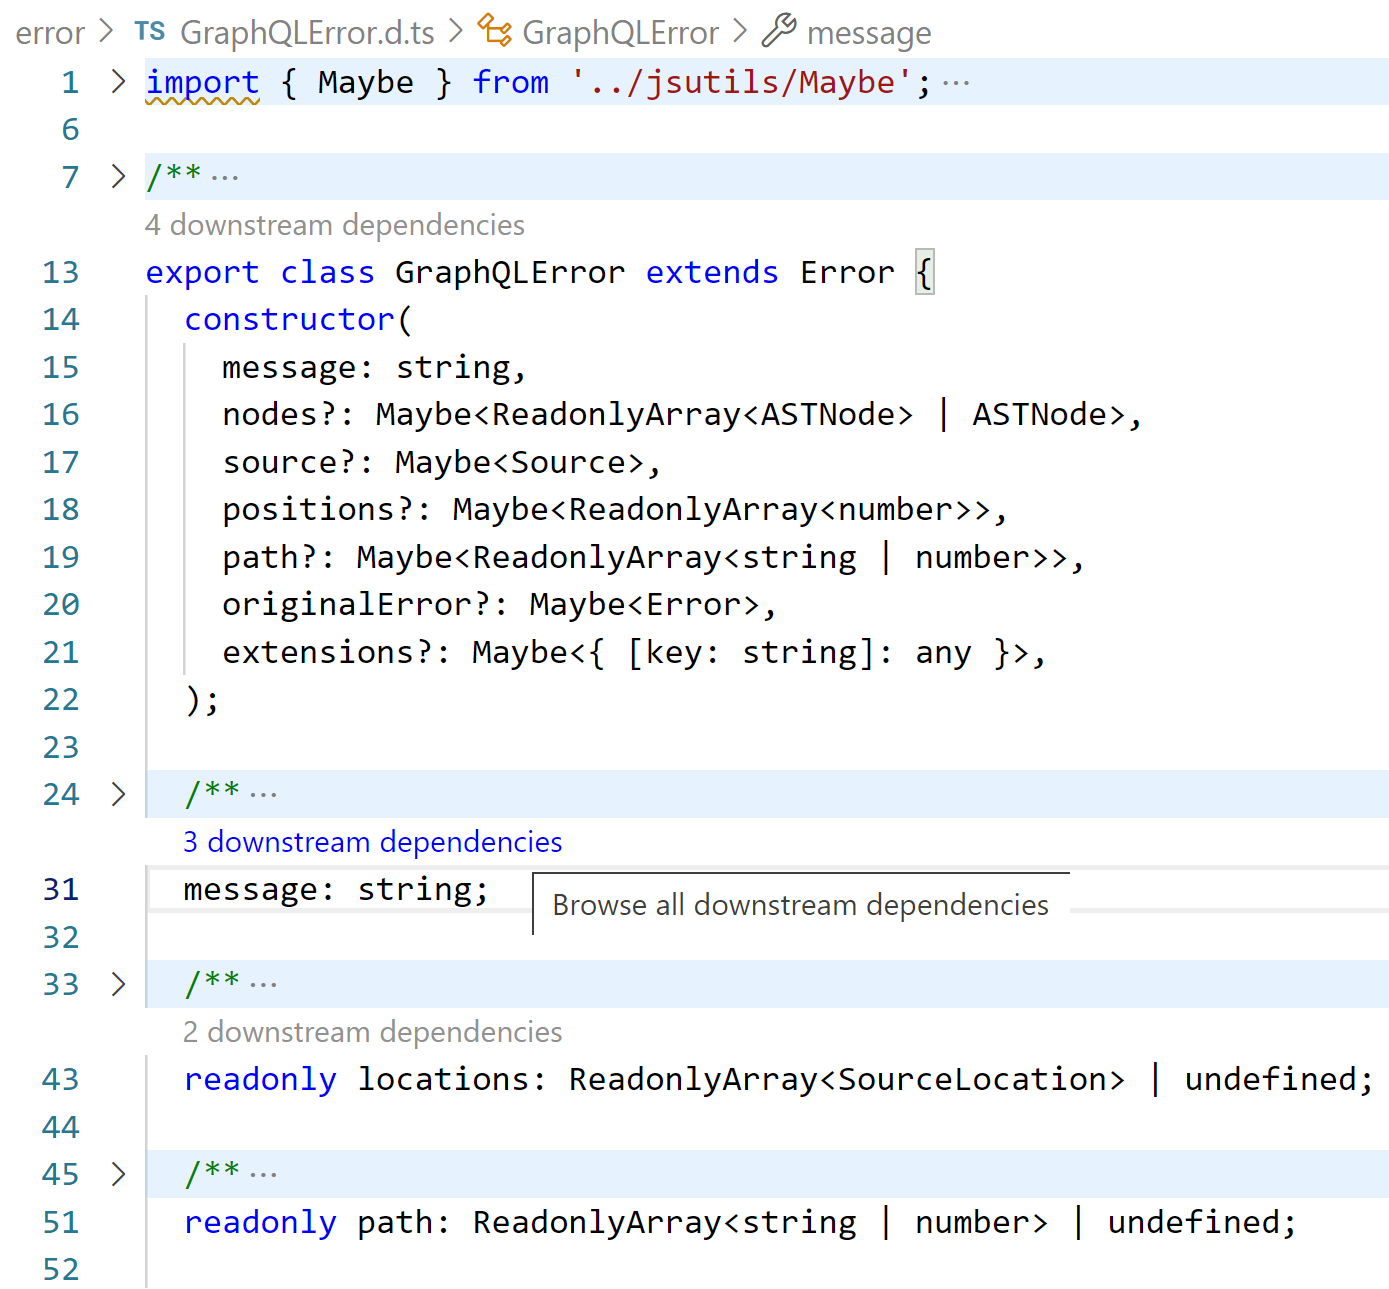
\includegraphics[width = 0.4288\dimexpr(\textwidth-2.0\pfull) - 0.25\pfull]{figures/codelens-cropped}};
        % sub-captions/labels:
        \node[below right = 0 of fig0, labelSE](lab0){(a) The dependency browser.};
        \node[below right = 0 of fig1, labelSE](lab1){(b) The usage browser.};
        \node[below right = 0 of fig2, labelSE](lab1){(c) The CodeLens integration for the class \texttt{GraphQLError}.};
        % spies:
        \spy on ($(fig2.center)+(-14.8mm, +20mm)$) in node at ($(fig2.center)+(+9mm,+1mm)$);
    \end{tikzpicture}
    %
    \caption{Screenshots of our VS Code extension used to explore downstream dependencies of the npm package \texttt{graphql}.}
    \label{fig:implementation/presentation/screenshots}
    %
\end{figure*}

Normally, foreign types can only be resolved if they are declared in a dependency module that has been installed into the \mycode{node_modules} folder of the repository.
Because downloading and installing all dependency modules for every downstream repository of the target package would increase the computational resources of the usage mining drastically and eventually violate \cref{req2}, we skip this step but instead modify the module resolution strategy of the TypeScript compiler host.
To do so, we extend the \mycode{paths} parameter from the default compiler options\footnote{\url{https://www.typescriptlang.org/tsconfig\#paths}} and insert a new entry that remaps accesses to the target package name to the separate source code directory of the target package.

\subsection{Presentation of Results}
\label{sec:implementation/presentation}

After all references have been collected, a proper user interface (UI) is still required to provide users easy access to these data that fulfills the requirements mentioned above.
To satisfy \cref{req1} and \cref{req3} by making our tool available in the usual working environment of users, we implement it as an extension to the \emph{Visual Studio Code} IDE\footnote{\url{https://code.visualstudio.com/}}.
It also provides a comprehensive set of APIs for extension developers.
To support other researchers in reusing our solution, we also provide a CLI.
The user interface is divided into three key views, supporting developers in answering the questions raised in \cref{sec:approach} (see \cref{fig:implementation/presentation/screenshots}):

\begin{enumerate}[label=(\roman*)]
	\item The \emph{dependency browser} allows to explore all downstream dependencies and, grouped for each dependency, all references to the target package.
	\item The \emph{usage browser} displays all public package members and, grouped for each member, all dependencies and their references to this member.
	\item The \emph{CodeLens integration} provides quick access to a slice of usage samples and is attached to the definition of each package member in the source code editor.
\end{enumerate}


Both references and members are organized each in a tree view that reflects the hierarchical structure of the original software repository.
In addition, we recognize the effort of browsing large lists of dependency data and encounter it by providing an \enquote{I'm feeling lucky} button for every view that redirects the user to a random dependency or reference, respectively, to gain a faster, unbiased impression of usage samples.

To implement each of these views in the VS Code Extension API (VSCE)\footnote{\url{https://code.visualstudio.com/api}}, we use the \emph{Tree View API} and the \emph{CodeLens API}.
One challenge has been to deliver fast results and not to block the user interface because even despite the lightweight mining methods we chose to satisfy \cref{req2} from above, querying, downloading, and analyzing each dependency takes a few seconds (see \cref{sec:evaluation}).
To overcome this issue, we use pagination wherever possible and push incremental UI updates. % apply the observer pattern to
As the VSCE API per se does not provide for multithreading or multiprocessing operations but suggests a Promise/A+-driven dataflow, we adopt this style for our object model by using the JavaScript concepts asynchronous functions, \mycode{AsyncIterator}s, and \mycode{Promise.all} to avoid busy waiting during the data collection process.



\begin{table*}[t]
    \centering
    \footnotesize
    \rowcolors{2}{white}{gray!15}%
    \setlength{\tabcolsep}{10pt}
    \setlength\aboverulesep{0pt}
    \setlength\belowrulesep{0pt}
    \renewcommand{\arraystretch}{1.45}
    \caption{Quantity and false-positive rates~(FPR) of downstream dependencies found by the presented methods (using npm and Sourcegraph) for selected packages.}
    \label{tab:evaluation/resqu1/quantities}
    \begin{tabularx}{0.9\linewidth}{Xcrcrcrrcrr}%
        %
            \toprule
            \rowcolor{white}
            \multicolumn{1}{c}{}
            & & &
            & \multicolumn{2}{c}{\textbf{npm}}
            &
            & \multicolumn{2}{c}{\textbf{Sourcegraph}}
            &
            & \\
        %
            \rowcolor{white}
            \textbf{Package}\rot{\hspace{5.5em}}
            &
            & \multirow[b]{-2}{*}[17pt]{\rot{GitHub stars}}
            &
            & \rott{c}{\strut Count}     %
            & \rott{c}{\strut FPR}  %
            &
            & \rott{c}{\strut Count}    %
            & \rott{c}{\strut FPR}    %
            &
            & \multirow[b]{-2}{*}[31.5pt]{\rot{Intersection in \%}}
            \\\toprule
        %
        base64id          & & \numprint{   16} & &  27 & 0.20 & & \numprint{  45} & 1.00 & & 8 \\
        nemo              & & \numprint{   38} & &   1 & 0.00 & & \numprint{   1} & 1.00 & & 0 \\
        random-js         & & \numprint{  556} & & 219 & 0.14 & & \numprint{ 193} & 0.36 & & 15 \\
        kubernetes-client & & \numprint{  902} & &  36 & 0.13 & & \numprint{  79} & 0.21 & & 16 \\
        jsonschema        & & \numprint{ 1547} & & 394 & 0.00 & & \numprint{ 517} & 0.18 & & 2 \\
        graphql           & & \numprint{18005} & & 396 & 0.17 & & \numprint{8863} & 0.68 & & 2 \\
        cheerio           & & \numprint{24228} & & 396 & 0.07 & & \numprint{6779} & 0.07 & & 0 \\\bottomrule
        %
    \end{tabularx}%\vspace{2mm}
\end{table*}



\section{Evaluation}
\label{sec:evaluation}

To evaluate our approach, we formulate three research questions:

\begin{enumerate}[label=RQ\arabic*,itemindent=0.3cm]
	\item \label[research question]{resqu1} What is the quality and quantity of the proposed methods for dependency collection?
	\item \label[research question]{resqu2} What is the quality and quantity of the proposed method for mining usage samples?
	\item \label[research question]{resqu3} How well is the proposed tool applicable with regard to the questions and requirements described in \cref{sec:approach}?
\end{enumerate}
%
In the following, we will investigate each question.

\subsection{\ref{resqu1}: Dependency collection}
\label{sec:evaluation/resqu1}

To assess the quality and quantity of dependency collection, we analyze it with respect to extent, precision, recall, and performance.
\Cref{tab:evaluation/resqu1/quantities} shows the number of dependencies collected to build an experimental dataset from each data source following the proposed methods for a set of manually selected npm packages.
For each package, we have annotated a subset of the collected dependencies (max. 20 dependencies per package) to identify and classify false positive hits.



\paragraph{Extent.}
\label{sec:evaluation/resqu1/extent}

Regarding the total number of dependencies collected by each method, no clear trend in favor of any method can be ascertained for small or medium packages, i.e., having less than \num{10,000} stars on GitHub.
For larger packages, i.e., having at least \num{10,000} stars, however, the number of dependencies collected from the npm registry stagnates near to 400 hits.
Beyond this limit, the npm registry returned internal server errors for our requests.
For Sourcegraph, we have not hit any limitations so far.
Currently, they do not provide any official documentation for the exact rate limits.
%
As the disjunct proportion of results from both methods is very small (on average about \SI{6}{\percent}), we consider a combination of both data sources useful for maximizing the extent and diversity of the gained dataset.

\paragraph{Precision.}
\label{sec:evaluation/resqu1/precision}

The precision of collected dependencies is drastically lower for dependencies found on Sourcegraph than for such found on npm.
\Cref{fig:evaluation/resqu1/fp_causes} collates the causes we have identified for false positives; most frequently, repositories specify a dependency on a target package in their package manifest file but do not import this package at any place.
%
\begin{figure*}[t]
	\centering
    %\small
    \footnotesize
	% Fix font size of \thead

    \pgfplotstableread[col sep=comma,]{measurements/fpr.csv}\datatable%
    \pgfplotstablefilter[source equals {Sourcegraph}]{\datatable}{\datatableSourcegraph}%
    \pgfplotstablefilter[source equals {npm}]{\datatable}{\datatableNpm}%
    \begin{tikzpicture}[outer sep=0pt]%
        \begin{axis}[
        	compat=newest,
        	name=fpr,
        	xbar=2pt,
        	axis on top,
        	%scaled ticks=true,
        	scaled x ticks=false,
        	width=0.8\linewidth,
        	height=14\baselineskip,
        	%enlarge x limits=0.15,
        	bar width=6.0pt,
        	%ylabel=\footnotesize{Types},
        	xlabel=\footnotesize{false-positive frequencies},
        	xmajorgrids,
        	major grid style={draw=white},
        	tick label style={font=\footnotesize},
        	xticklabel style={
        		/pgf/number format/fixed,
        		/pgf/number format/precision=2
        	},
        	axis x line*=bottom,
        	axis y line*=left,
        	xtick align=outside,
        	%ytick={0,2,...,14},
        	%ytick=data,
        	yticklabels={,package unused,peer dependency,type definitions only,package.json mismatch},
        	xmin=0.0,
        	xmax=0.45,
        	ymin=-0.5,
        	ymax=3.5,
        	point meta=rawx,
        	nodes near coords,
        	every node near coord/.append style={anchor=west, font=\footnotesize,/pgf/number format/.cd, precision=2, fixed,1000 sep={\,}},
	        %nodes near coords align={vertical},
    	]
    	    \addplot[white,very thin,fill=plots-1,text=black] table[x={fpr},y expr=\coordindex]{\datatableSourcegraph};
    	    \addplot[white,very thin,fill=plots-2,text=black] table[x={fpr},y expr=\coordindex]{\datatableNpm};
    	\end{axis}
    	\begin{axis}[
        	name=fpr_legend,
        	compat=1.3,
        	at={($(fpr.north east)+(0.0cm,0.0cm)$)},
        	hide axis,
        	bar width=0pt,
        	ticks=none,
        	%legend columns=2,
        	legend style={
        		at={(0.0,0.0)},
        		anchor=north east,
        		draw=none,
        		legend cell align=left,
        		%/tikz/column 2/.style={
                %    column sep=5pt,
                %},
        	},
        	legend image code/.code={%
        		\draw (0.0cm,-0.05cm) rectangle (0.4cm,0.15cm);
        	},
        	text height=1.1ex,
        	%width=0.5\columnwidth,
        	height=2cm,
        ]
        	\addplot[draw=none,white,very thin,fill=plots-1] coordinates {(0,0)};
        	\addlegendentry{\; Sourcegraph}
        	\addplot[draw=none,white,very thin,fill=plots-2] coordinates {(0,0)};
        	\addlegendentry{\; npm}
        \end{axis}%
    \end{tikzpicture}%
    %\vspace{-1\baselineskip}
	\caption{Causes for false-positive dependency matches and their frequencies.}
	\label{fig:evaluation/resqu1/fp_causes}
\end{figure*}
%
In some situations, this may happen if the package is a plugin for another package or if it is invoked as a CLI from a build script, but in the majority of repositories, developers trivially appear to have specified the upstream dependency by accident (e.g., while copying a \mycode{package.json} file over from another package), or to have forgotten to remove the upstream dependency after switching away from using the package.
Less common causes are repositories that only add type definitions to a package but do not actually import it, as well as packages required by a repository that declares a peer dependency on the target package, which needs to be fulfilled by the depending repository.
%
We explain the increased false-positive rate for Sourcegraph dependencies by our observation that packages found on npm are deliberately published and typically stand out by their higher cohesion and commitment to maintenance, whereas GitHub-only projects contain a higher share of hobby or students' projects.
%
We stress that a reduced precision does not impair the quality of results displayed to package developers as all dependencies not containing at least one
usage sample can be easily filtered out, but downloading and analyzing any irrelevant packages lowers the performance of the approach.

\paragraph{Recall.}
\label{sec:evaluation/resqu1/recall}

Besides the precision of the collected dependencies, their recall is of interest, too.
Since dependencies are collected in excerpts from two large datasets, a quantitative analysis of false negatives would require costly manual annotation and is target for future work.
Nevertheless, some causes will prevent a dependency from being found by our methods:

\begin{table*}
    \footnotesize
    \centering
    \rowcolors{2}{white}{gray!15}%
    \setlength{\tabcolsep}{25pt}
    \setlength\aboverulesep{0pt}
    \setlength\belowrulesep{0pt}
    \renewcommand{\arraystretch}{1.45}
    \caption{Performance metrics and remarks for both dependency collection methods using npm and Sourcegraph.}
    \begin{threeparttable}
        \begin{tabularx}{0.9\linewidth}{Xrr}
            \toprule
            \textbf{Metric}                       & \textbf{npm} & \textbf{Sourcegraph} \\\midrule
            \strut Search speed~\textsuperscript{a} \hfill\si{\second/pkg}
                & 1.58 &  0.04  \\
            \strut Download speed~\textsuperscript{a,b} \hfill\si{\second/pkg}
                & 0.26 &  8.80  \\
            \strut Storage \hfill\si{\mega\byte/pkg}
                & 5.80 & 27.20  \\
            \strut API limitations & max. 400 results & none known\\ \bottomrule %
        \end{tabularx}
        \begin{tablenotes}\footnotesize
            %
    		\item[\textsuperscript{a}] Test machine: 7 vCPUs Intel Xeon Cascade Lake at
    		\SI{2.80}{\giga\hertz}, internet down speed \SI{1.8}{\giga\bit/\second}.
    		%
    		\item[\textsuperscript{b}] Effective speed downloading multiple packages in parallel to manage latencies.
    		%
        \end{tablenotes}
    \end{threeparttable}
    \label{tab:evaluation/resqu1/performance}
\end{table*}

\begin{itemize}
	\item Packages without a proper dependency manifest cannot be detected as our method is based on parsing these metadata.
	\item Only published packages are found on npm, leading to a bias for generic and professional software.
	\item On both platforms, results will be sorted based on intransparent criteria (which, as we speculate, include the number of direct dependents on npm and the recent update frequency on Sourcegraph, respectively).
	As we only fetch the first dependencies from both data sources, this is a likely source of further biases.
	These biases could be fought by always fetching all dependencies, but this would drastically reduce performance and would require a workaround for the npm query limitation.
\end{itemize}


\paragraph{Performance.}
\label{sec:evaluation/resqu1/performance}
\Cref{tab:evaluation/resqu1/performance} gives some basic metrics comparing the performance of both data sources.
While searching downstream dependencies is slower by average on npm as we use a web scraper instead of an API for this source, npm packages are usually smaller than many mono-repositories on OSS platforms that contain multiple node.js packages.
In addition, they are faster to download since the \texttt{download-git-repo} package that we use for repositories found on Sourcegraph only uses zipballs instead of tarballs (\texttt{.tar.gz} files), while the latter would offer a higher compression rate.


\subsection{\ref{resqu2}: Usage mining}
%
To assess the quality and quantity of usage mining, we examine this processing step's precision, recall, and performance.
Due to the complexity of a detailed annotation process, we only consider the existence of found usage samples on the dependency level.
The absolute quantity of found usage samples largely varies for different packages and dependencies based on the semantic extent of the package and the coupling.% between package and dependency.


\paragraph{Precision.}
%
Under laboratory conditions, false-positive usage samples cannot be emitted by our method if we assume the correctness of the TypeScript compiler.
There are only two theoretical exceptions to this invariant:
%
\begin{enumerate*}[label=(\roman*)]
    %
	\item In case of a name collision between two packages, invalid or false positive usage samples may be emitted.
        However, the npm infrastructure attempts to rule out these collisions by using the package name as a unique ID for every published package.
	%
	\item If dependency developers deliberately interfere with the TypeScript compiler (for instance,
	    by suppressing type errors using \texttt{@ts-ignore} comments, both false positive and false negative matches are possible.
	%
\end{enumerate*}
%
Additionally, some npm packages contain minified sources only that are still searchable, valid code but can be significantly harder to read.

\paragraph{Recall.}
%
To evaluate the recall of our method, we have refined the experimental dataset collected in \cref{sec:evaluation/resqu1} and removed all false-positive dependencies.
Within this cleansed dataset, the overall rate of dependencies for that our method cannot find at least one usage sample accounts for \SI{47.9}{\percent}.
To explain these false negatives, we have identified some systematic causes:
%
\begin{itemize}
    %
	\item Many projects on OSS platforms have complex build configurations that include additional transpilation or code generation steps before a final version of the source code is reached that is valid to the node.js interpreter or the TypeScript compiler.
		Unless we add explicit support for such build configurations, type analysis and usage mining for these projects will fail.
	%
	\item In some situations, additional type definitions are required to perform a complete type inference of a dependency.
		This applies to every parametrized callback from a package for that type definitions are not available.
		This limitation could be resolved by downloading or generating type definitions for all upstream dependencies of every downstream dependency; however, this would reduce the approach's performance.
	%
	\item The static type analyzer of TypeScript has some limitations.
		For instance, the type analysis will have a limited recall for certain control flow patterns or metaprogramming constructs such as meta-circular evaluation using the \texttt{eval()} function or dynamic function binding using \texttt{Function.bind()}.
		These limitations could be resolved with AST preprocessing and partial evaluation of the source code.
	%
\end{itemize}


\paragraph{Performance.}
%
The total time spent performing type analysis for a repository from the experimental dataset and mining usage samples averages about \num{3} seconds.
The complete ASF of an average parsed repository consumes between \SI{10}{\mega\byte} and \SI{500}{\mega\byte} memory, depending on the size of the repository.



\subsection{\ref{resqu3}: Requirements}
\label{sec:evaluation/resqu3}
%
To assess the applicability of our tool, we investigate different options for users who would like to answer the questions raised in \cref{sec:approach}.
We further analyze how far our tool meets the requirements posed above.


\paragraph{Answering User Questions.}
%
To answer \cref{q1} without our tool, users could access the data sources used by our tool manually to search for and view downstream dependencies.
The source code of repositories can be browsed on Sourcegraph, but if an npm package is not available on an OSS platform, users will need to download and extract it.
With our tool, the data collection process is condensed into a single button that incrementally displays all references from both data sources.
Users can hover or click any dependency to view its documentation or implementation.
%
To answer \cref{q2,q3} without our tool, users need to scan each found dependency separately to count or read all usage samples.
If they intend to analyze the usage of a member with an exact name, they can perform an expeditious string search.
This is possible using Sourcegraph or another search engine if the dependency is indexed there; otherwise, users will need to download the repository and search it locally.
If the member of interest has an ambiguous name, users will need to download the project and view it in an IDE such as VS Code that supports reference search.
Alternatively, they can try the precise code intelligence mode on Sourcegraph (see \cref{sec:related_work/usage_samples}); however, this feature is available for a few repositories only.
%
All usage samples can be collected automatically and merged into a single list within our tool.
Once the collected dependencies have been processed, users can select a member of interest and view all its usage samples with a single click.
For the usage analysis of Java APIs, the tool \emph{Exapus} also considers different kinds of member usages such as instantiation vs. inheritance of a class \cite{de2013multi}; a similar classification could improve the usability of our tool.


\paragraph{Meeting Requirements.}
%
To satisfy \cref{req1}, the application needs to be easy to set up.
As our extension can be installed with two clicks from the Visual Studio Code Extension Marketplace and the installation takes less than 10 seconds on our test machines, it fulfills this requirement.

We break down \cref{req2} into two acceptance criteria: application liveness and small resource footprint.
As discussed before, our tool can process 5 up to 12 dependencies per minute while requiring about \SI{500}{\mega\byte} memory in total and less than \SI{30}{\mega\byte} storage per package.
After the tool is activated, the first results usually appear after less than 10 seconds on the UI.
This is an acceptable delay regarding Shneiderman's definition of acceptable application response times, so the liveness criterion is fulfilled.
Even if the tool downloads a few hundred dependencies, it will occupy less than \SI{10}{\giga\byte} storage that can be released at any time, which we consider a small resource footprint at a time where modern operating systems require \SI{64}{\giga\byte} storage; thus, the second criterion is fulfilled as well.

\Cref{req3} effectively calls for a minimum number of context switches that are required to use the tool, i.e., for minimizing the temporal, spatial, and semantic distance~\cite{ungar1997debugging} between the downstream dependency UI and the IDE used by package developers.
%
Once the data are available in the UI, interaction is possible with the same speed as with local source files in the package.
This meets Shneiderman's requirement to frequent tasks and indicates a low temporal distance.
%
The spatial distance varies for the different views of the tool:
A separate toolbar has to be opened for the dependency and usage browsers, which indicates a higher spatial distance; still, the artifacts are available in the same IDE.
Also, the dependency artifacts have no strong relation to any existing IDE artifacts, so any closer integration into an existing view would increase coupling between independent domains.
The code annotations are displayed close to the package source code with a small spatial distance.
%
The semantic distance can be described as the perceived similarity of artifacts displayed both in the tool's UI and in the existing IDE, i.e., the package and dependency members.
Most items in the usage browser bear the same label as the corresponding identifier in the source code, which reduces the semantic distance.
However, dependency member path nodes that refer to anonymous expressions are displayed differently compared to the outline view of VS Code (see \cref{fig:implementation/presentation/screenshots} (a)), slightly increasing the semantic distance.
%
With a low temporal distance, a low-to-medium spatial distance, and a mainly low semantic distance, our tool also fulfills \cref{req3}.




\section{Conclusions and Future Work}
\label{sec:conclusion}

Downstream dependencies offer a promising perspective for package developers interested in understanding how their interfaces are used in practice by other software developers.
In this paper, we have proposed an automated approach to making this sort of information accessible to package developers by automating the dependency collection and mining of usage samples from every dependency.
We have identified two kinds of rich data sources for efficiently collecting downstream dependencies: public package repositories, such as npm, and online code search engines for finding dependent repositories by their package manifest files, namely Sourcegraph.
We accomplish the usage mining by scanning the ASTs of every dependency for certain usage patterns that refer to a type from the target package; if the dependency uses a dynamically typed language, we perform a type analysis before.
We have demonstrated the usability of our approach with a tool that embeds the downstream dependency data into the VS Code IDE.
%
Our analysis suggests that the collected dependencies and the extracted usage samples have a viable quality in terms of precision and extent and further that the resource requirements of our prototype are sufficiently low for collecting all data on the local machine of a package developer.

Nevertheless, we have identified several causes for false negatives over the whole mining process that can bias the output usage samples, including the popularity and recency of dependencies but also the proper declaration of packages and their renunciation of complex toolchains and metaprogramming patterns.
Our analysis, however, is not yet fully supported by data and would require further quantitative evaluation to assess the exact precision and recall of our approach for mining usage samples as well as the efficacy of our tool.
As for the first question, manual annotation of source code repositories with usage samples will be required to compare them to the outputs of our implementation.
Close insights for the second question could be gained from a user study that measures the impact of our tool on the efficiency of package developers solving downstream dependency-related tasks.

We believe that our tool has further potential to support package developers in surveying downstream dependencies.
As future work, we envision other purposes for analyzing the collected downstream dependency data, including usage pattern mining, automated convenience protocol suggestions, and the generation of metrics for classifying downstream dependencies or measuring the cohesion and impact of libraries within an ecosystem.
By extending the static usage analysis with a dynamic approach, the detected usage samples could be enriched with valuable runtime data describing involved parameters, the fine-grained code coverage of package members, or the invocation context of members.
Returning to the abstract problem that we have formulated in the introduction -- how can we improve developer knowledge about their packages' usage? --, further data sources next to source code files emerge that could be mined for package references, too.
For instance, we are looking forward to solutions that mine the change history of projects for package-related changes (potentially indicating breaking changes), search conversation platforms such as public issue trackers or Q\&A forums for mentions of package members and analyze their sentiments, e.g., potentially indicating confusing behavior or bad documentation), or even scan continuous integration logs for failure stack traces (e.g., potentially revealing bugs in the package of interest.



\section*{\uppercase{Acknowledgements}}

We want to thank the anonymous reviewers for their valuable comments and suggestions to improve this article.
This work is part of the \enquote{Software-DNA} project, which is funded by the European Regional Development Fund (ERDF or EFRE in German) and the State of Brandenburg (ILB).
This work is also part of the KMU project \enquote{KnowhowAnalyzer} (Förderkennzeichen 01IS20088B), which is funded by the German Ministry for Education and Research (Bundesministerium für Bildung und Forschung).


\bibliographystyle{apalike}
{\small%\balance
\bibliography{paper}}


\end{document}
